% Usar el tipo de documento: Artículo científico.
\documentclass[10pt,a4paper,hidelinks]{article}

% Cargar mensajes en español.
\usepackage[spanish,es-noquoting]{babel}

% Usar codificación utf-8 para acentos y otros.
\usepackage[utf8]{inputenc}
\usepackage[T1]{fontenc}
\usepackage{lmodern}

% Dimensiones de los márgenes.
\usepackage[margin=1.8cm]{geometry}

% Insertar porciones de código
\usepackage{listings}

% Comenzar párrafos con separación no indentación.
\usepackage{parskip}
%enlaces
\usepackage{hyperref}
% Usar gráficos
\usepackage{graphicx}
\usepackage{caption}
\usepackage{subcaption}
%
% Usar contenedores flotantes para figuras.
\usepackage{float}

% Carpeta de las imágenes.
\graphicspath{{img/}}

% Matemáticas
\usepackage{amsmath}
\usepackage{mathtools}

% Símbolos del sistema internacional
\usepackage{siunitx}

% Gráficas con pgf
\usepackage{pgfplots}

% Tablas con varias filas unidas
\usepackage{multirow}

% Tablas en el texto
\usepackage{wrapfig}

\begin{document}
%\maketitle
\begin{center}
\begin{huge}
\textbf{Trak}
\end{huge}
\\[10pt]
\textbf{Rodrigo Arias Mallo}\\
rodrigo.arias@udc.es
\end{center}

\section{Diseño artístico}
\section{Descripción}
Trak es un videojuego 3D de conducción extrema. Las altas velocidades, los 
saltos en el aire, o las pendientes perpendiculares son habituales en las 
carreras.

Está ambientado en la serie de videojuegos TrackMania. Los aspectos de 
conducción así como el modelo de pistas siguen el mismo estilo.

\section{Diseño interno}
\subsection{Introducción}
El juego está íntegramente desarrollado en Blender, un editor de modelos 3D, que 
incluye un motor gráfico basado en el motor de físicas Bullet.

\subsection{Vehículo}
\subsubsection{Estructura}
El vehículo está formado de una parte estética, que se mostrará en el juego, y 
una representación más simple, empleada en las físicas.

En la parte estética se encuentra la carrocería, y las cuatro ruedas que tienen 
desactivada la colisión con otros objetos. Además han sido simplificados 
estructuralmente, para acelerar el renderizado. De esta forma los 215.000 
vértices se reducen a un 16\%: 35.000.

La estructura que se muestra a continuación proporciona la simplificación 
adecuada para realizar colisiones con el vehículo sin la complejidad de la 
carrocería.

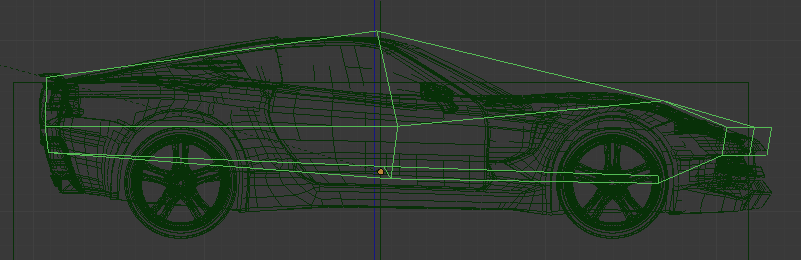
\includegraphics[width=\textwidth]{vehiculo-colision}

\subsubsection{Control}
El control del vehículo se realiza mediante un controlador de vehículos que 
incluye Bullet. De esta forma se simplifica la hercúlea tarea de simular el 
comportamiento de un coche, a una tarea compleja; la de ajustar el 
comportamiento al de un coche real.

Existen diferentes parámetros que configuran el control del vehículo.

\begin{wraptable}{l}{5cm}
\begin{tabular}{ | c | l | }
	\hline
	\multirow{2}{*}{Fuerza}
	& Motor \\
	& Frenos \\
	\hline
	\multirow{4}{*}{Suspensión}
	& Rigidez \\
	& Amortiguación \\
	& Longitud \\
	& Compresión \\
	\hline
	\multirow{3}{*}{Ruedas}
	& Radio \\
	& Fricción \\
	& Influencia \\
	\hline
	\multirow{3}{*}{Vehículo}
	& Dimensiones \\
	& Masa \\
	& Gravedad \\
	\hline
\end{tabular}
\end{wraptable}

Fuerza del motor, fuerza de los frenos
Rigidez






\end{document}
